\documentclass[]{article}
\usepackage{graphicx}
\usepackage{hyperref}
\usepackage{amsmath}
\usepackage{caption}
\usepackage{subcaption}
\usepackage{ngerman}
\usepackage[utf8]{inputenc}
\usepackage{float}

%opening
\title{Hochauflösende $\gamma$ Spektroskopie}
\author{Gunther T\"urk, Jonas Lehnen}

\begin{document}

\maketitle
\begin{abstract}
In diesem Experiment wollen wir verstehen wie der $\gamma$ Zerfall gemessen wird um die genaue Energie des Photons zu bestimmen. Nach dem ein Elektron gefangen oder ein $\beta$ Zerfall statt fand, ist der Atomkern angeregt. Die Abregung des Kerns erfolgt über eben dieses Photon, welches ein Germanium Detektor messen kann. In diesem Zuge werden wir besprechen in wie weit Elektronik und Hintergrundstrahlung dieses Experiment beeinflussen.
\end{abstract}

\tableofcontents


\newpage
\section{Theorie}
\subsection{Radioaktive Strahlung}
Grundsätzlich existieren drei Arten des radioaktiven Zerfalls. Beginnend mit dem $\alpha$ Zerfall, bei dem ein ${He}\ ^{2+}$ Teilchen aus einem größeren Atomkern emittiert wird. Die genauen Zerfallskanäle sind in Tabelle \ref{tab:zerfall} dargestellt. $\alpha$ Strahlung selbst ist leicht abgeschirmt, so besteht bereits nach $10cm$ Luftweg keine Belastung für Menschen. Probleme entstehen erst bei Alphastrahlern im Körper, da dann die gesamte Energie deponiert wird und unter anderem Krebs auslösen kann.

\renewcommand{\arraystretch}{2}
\begin{table}[H]
\centering
\begin{tabular}{c||c}
Zerfallsart & Formel   \\ \hline
$\alpha$ & $_Z^A X \rightarrow\ _2^4\alpha + _{Z-2}^{A-4} Y$ \\ \hline
$\beta^+$ &   $_Z^A X \rightarrow\  _{Z-1}^{A}Y + e^+ + \nu_e$ \\ \hline
$\beta^-$ &   $_Z^A X \rightarrow\  _{Z+1}^{A}Y + e^- +  \bar{\nu}_e$ \\ \hline
$\gamma$ &  $_Z^A X^* \rightarrow\ _Z^A X + \gamma$  \\ \hline
$EC$ &   $_Z^A X  + e^- \rightarrow\ _{Z-1}^{A}Y + \nu_e $
\end{tabular}
\caption{Darstellung aller möglichen radiokativen Zerfälle. Die Kernendprodukte können sich, bis auf beim $\gamma$ Zerfall, noch in einem angeregten Zustand befinden. Dies wird durch $X^*\ bzw.\ Y^*$ dargestellt.  }
\label{tab:zerfall}
\end{table}
\renewcommand{\arraystretch}{1}

Wie in jedem Zerfall gilt auch für die $\beta$ Zerfälle, dass die Masse des ursprünglichen Kerns größer ist als die der Zerfallsprodukte. Dies liegt an der Energieerhaltung, da zusätzliche kinetische Energie entsteht um das Zerfallsteilchen fort zubewegen. Hier unterscheidet man je nach Ladung von Elektron oder Positron zwischen negativen um positiven $\beta$ Zerfall. Damit auch die Flavourerhaltung der Leptonen berücksichtigt wird, entstehen hierbei zusätzliche Neutrinos. Im Kern selbst zerfällt dabei ein Neutron bzw. Proton zu genau dem anderen Kernteilchen. Der Zerfall eines freien Protons ist theoretisch möglich jedoch wird die Halbwertszeit auf $10^{35}$ Jahre geschätzt. Unser Universum ist bisher erst ca. $10^{10}$ Jahre alt. Es ist also sehr unwahrscheinlich einen solchen Nachweis in einem Menschenleben erbringen zu können.

Alle genannten Strahlungsarten können nun in einem angeregten Kernzustand enden. An dieser Stelle setzt nun der $\gamma$ Zerfall ein. Diese angeregten Zustände sind durch Kernspin und Parität charakterisiert. Dieser Zerfall entspricht einer Umstrukturierung des Kernaufbaus und die dabei gewonnene Energie hat zwei Möglichkeiten umgesetzt zu werden. Entweder als Photon des $\gamma$ Zerfalls oder auch direkt an ein Elektron, welches dann das Atom verlassen kann, sofern die Bindungsenergie aufgebracht werden konnte. Dieser Prozess wird Innere Umwandlung genannt und kann nur mit Elektronen einer s-Schale stattfinden, da nur diese eine Aufenthaltswahrscheinlichkeit im Kern besitzen.

\begin{figure}[H]
\centering
\begin{subfigure}[b]{.48\textwidth}
\centering
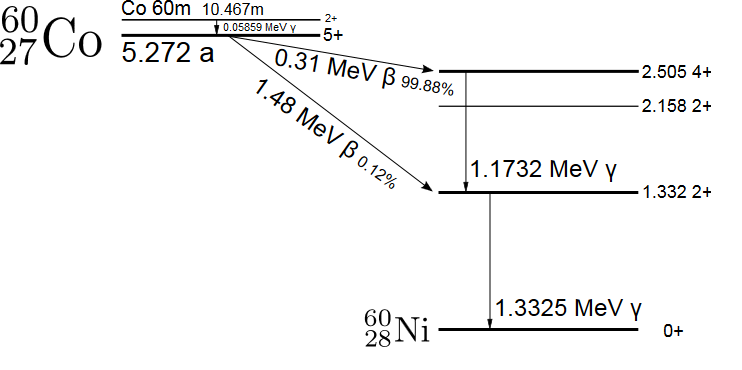
\includegraphics[width=1\textwidth]{Plots/Cobalt1.png}
\caption{Schema der Energieniveaus und Zerfallsübergänge. Vor dem eigentlichen $\gamma$ Zerfalls findet ein $\beta^-$ Zerfall statt. Am rechten Rand sind Kernspin und Parität vermerkt. Die Halbwertszeit ist mit mit 5.272 Jahren ebenfalls dargestellt.}
\end{subfigure}
\begin{subfigure}[b]{.48\textwidth}
\centering
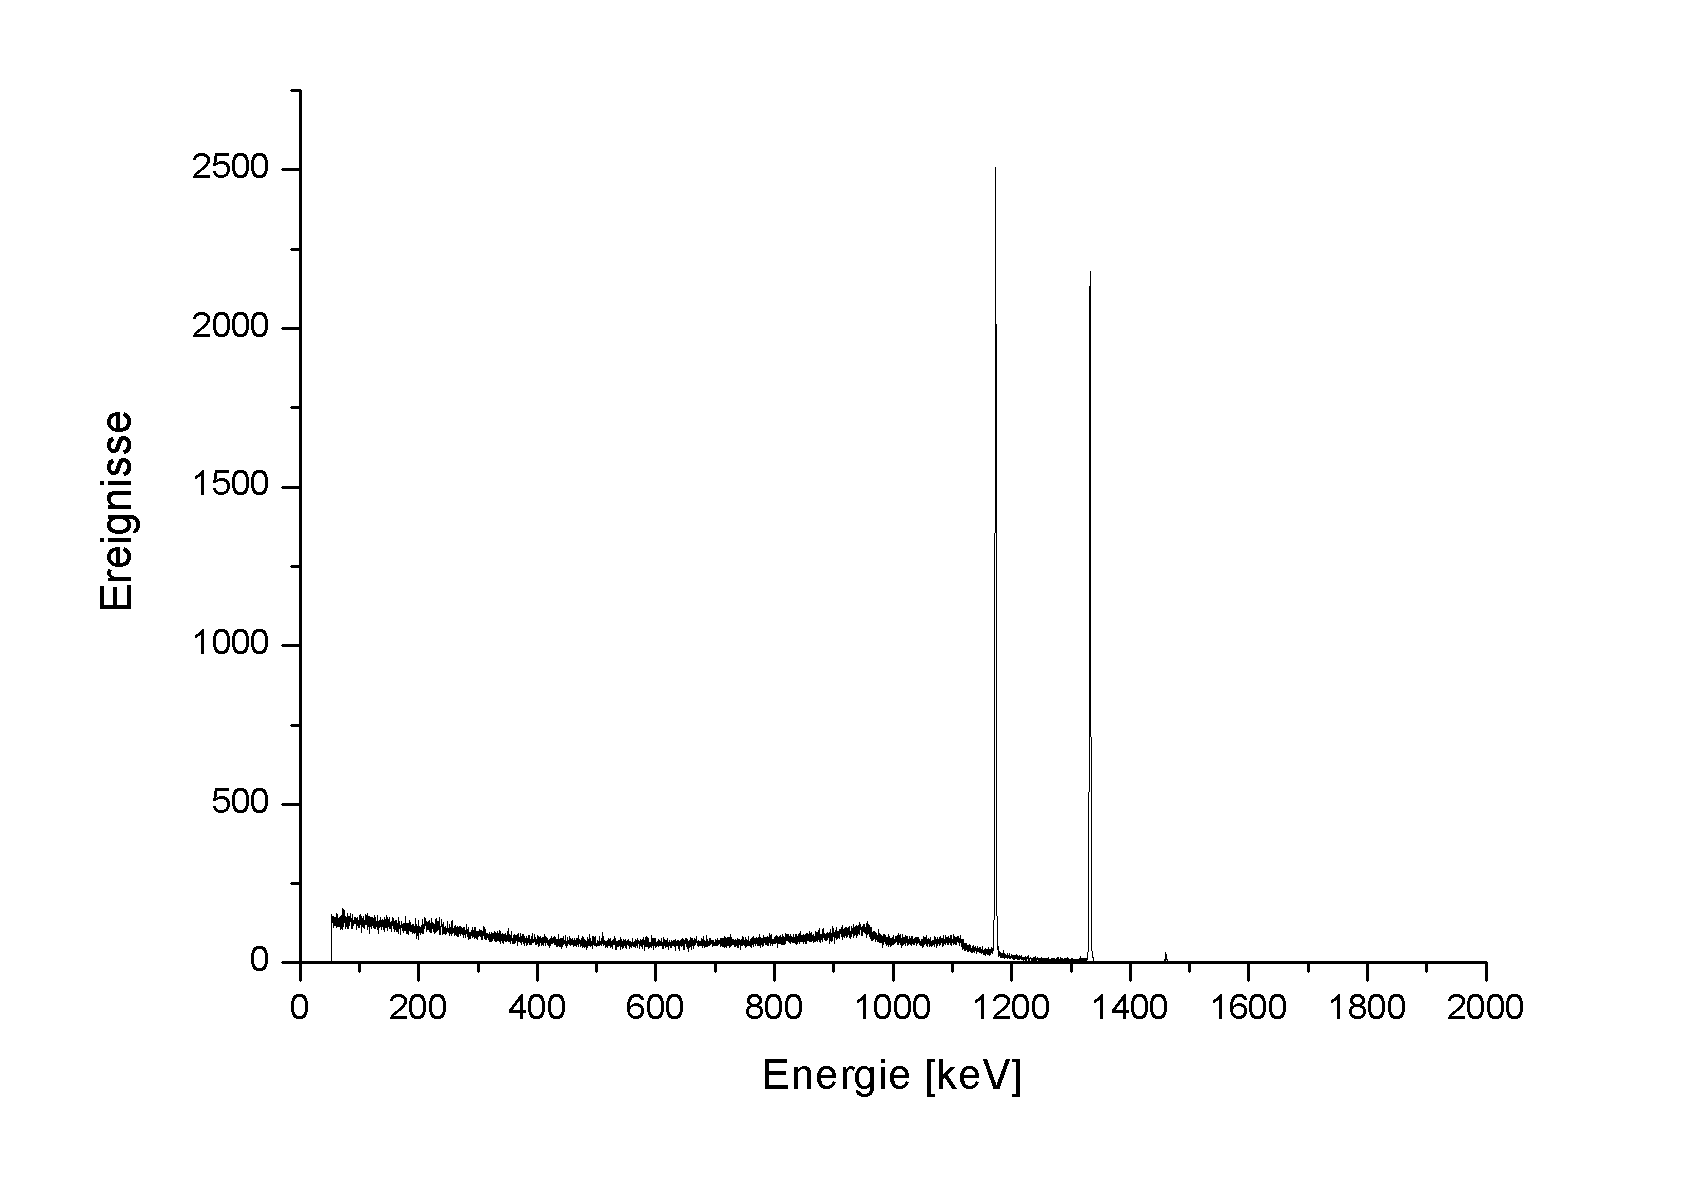
\includegraphics[width=1\textwidth]{Plots/Cobalt2.png}
\caption{Spektrum des $\gamma$ Zerfalls. Beide Peaks entsprechen den im $^{60}Ni$ angegebenen Energien des Übergangs. }
\end{subfigure}
\caption{Darstellungen des $\gamma$ Zerfalls vom $^{60}Co$. \cite{cobalt}}
\end{figure}

Zusätzlich existiert noch der Gegensatz zum $\beta$ Zerfall. Beim Electron Capture EC wird ein Elektron eingefangen statt ausgesendet. Durch die Änderung des Kerns befindet sich jetzt das gesamte Atom in einem angeregten Zustand, statt der Kern. Am wahrscheinlichsten ist, dass ein $e^-$ aus der K-Schale gefangen wird. Dabei entsteht ein freier Platz auf einem niedrigen Niveau, welcher dann von oben wieder nach besetzt wird. Dabei entsteht nun Röntgenstrahlung, statt $\gamma$ Strahlung. Der Unterschied zwischen besteht also darin, ob das Photon im Kern ($\gamma$) oder aus der Schale (Röntgen) stammt.

%%% Zur Vollständigkeit wird noch das Zerfallsgesetz angegeben?
%%% Aktivität dazu vll?


\subsection{Photonische Wechselwirkung mit Materie}
Je nach Energiebetrag eines Photons gibt es verschiedene Arte um mit Materie zu interagieren. Hauptsächlich geschieht die Wechselwirkung durch den Compton-Effekt. Dabei wird das Photon elastisch an meist einem Elektron gestreut, prinzipiell sind aber alle geladenen Teilchen denkbar. Das Elektron erhält zusätzliche kinetische Energie und die Wellenlänge des Photons erhöht sich. Dieser Effekt tritt bei fast allen Photonenenergien auf. Seine Wahrscheinlichkeit kann jedoch in bestimmten Regionen durch andere Effekte unterdrückt sein.

Der Photoeffekt ist einer davon. Er dominiert für geringere Energien bis ca. $500\ keV$. Bei diesem Prozess handelt es sich um die komplette Absorption von Energie und Impuls des Photons durch ein Elektron, welches dabei die Möglichkeit erhalten kann die Bindungsenergie zu überwinden. Überschüssige Energie findet sich im Impuls wieder.

Der andere Effekt, der für hohe Energien ab einigen $MeV$ dominiert, ist die Paarbildung. Hierbei besitzt ein Photon genug Energie um ein Elektron und ein Positron zu erzeugen. Da ein Photon sich in jedem Bezugssystem, also auch im Ruhesystem von $e^-,e^+$, mit Lichtgeschwindigkeit c bewegt, wird hierbei ein Kern benötigt um die Impulserhaltung zu gewährleisten. 

Alle diese Effekte führen dazu, dass sich meist ein Elektron mit überschüssiger Energie in der Materie bewegt. Dabei kann nun Bremsstrahlung auftreten. Es werden somit wieder Photonen frei und eine Kette aus diesem Prozessen findet statt. Dies ist der Grund warum im folgenden Kapitel überhaupt die Möglichkeit besteht radioaktive Zerfälle elektrisch wahrzunehmen.

\begin{figure}[H]
\centering
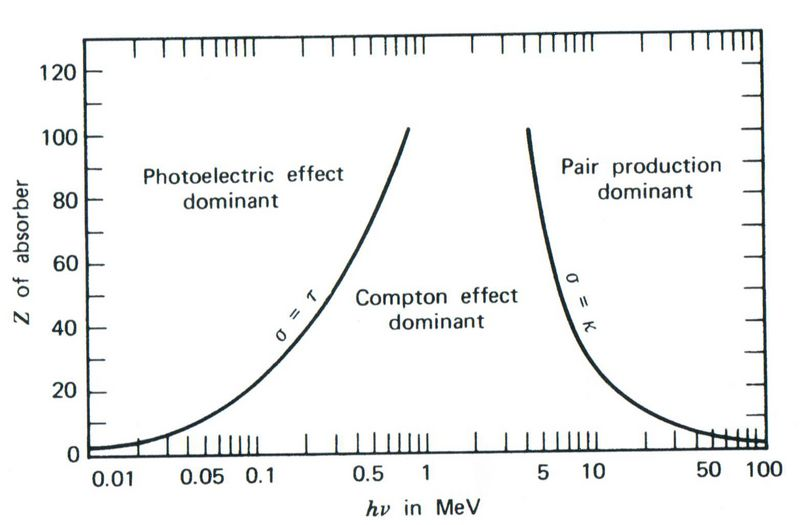
\includegraphics[width=.7\textwidth]{Plots/PhotonInteraktion.png}
\caption{Darstellung welche Interaktion der Photonen mit Materie in welchen Energiebereichen am wahrscheinlichsten ist. }
\end{figure}

\subsection{Detektion von Strahlung}
Es gibt nun je nach Verwendungszweck verschiedene Arten um Teilchen nachzuweisen, insbesondere auch um radioaktive Strahlung zu detektieren. Für die meisten Nachweise werden Szintillatoren verwendet. Das Prinzip besteht darin, dass das Strahlungsteilchen seine Energie an das Material des Szintillator abgibt und dabei Elektronen frei werden. Dies kann durch Streuprozesse als auch den Photoeffekt geschehen. Dieser spielt im zweiten Schritt eine große Rolle, da die freien Elektronen meist noch genug Energie besitzen um Bremsstrahlung zu emittieren. Durch die Wiederholung des Prozesses entsteht ein Lichtblitz der sich durch das Material fortsetzt. 

Zur digitalen Auswertung des Ereignisses wird dann ein Photomultiplier benötigt. Dieser beruht ebenfalls auf dem Photoeffekt, doch nun wird das frei Elektron von einer Anode angezogen, da diese auf einem höheren Potential liegt als die Anode, welche vom Photon getroffen wurde. Mit der aus dem elektrischen Feld gewonnenen Energie können nun an der Anode weitere Elektronen herausgeschlagen werden. Durch stets versetzte Anoden, damit die Elektronen keine Anode überspringen, nimmt deren Anzahl pro Anode exponentiell zu. Zum Schluss wird noch der Stromfluss gemessen, welcher proportional zur anfangs deponierten Energie ist. Diese Anwendung ist gut solange die genaue Energie eines Ereignisses nicht sonderlich wichtig ist sondern nur dessen Vorkommen und Aktivität. Sie sind jedoch besser als ein Geiger-Müller Zählrohr, bei dem nur die Anzahl der Teilchen messbar ist.

Um eine genaue Energieauflösungen zu erhalten, welche den Sinn der hochauflösenden $\gamma$ Spektroskopie darstellen, sollte man nun Halbleiterdetektoren benutzen. Hierbei 
werden statt Szintillatoren Halbleiterbauteile benutzt. In diesem Experiment wird wie auch meist ein koaxialer Germanium Detektor verwendet. Das Prinzip dahinter ist die Verwendung der Sperrschicht, welche entsteht wenn verscheiden dotierte Versionen eines Halbleiters aneinander geführt werden. Der Überschuss von Elektronen im n-dotierten Material wird vom Mangel an $e^-$, bzw. Überschuss an Löcher, abgesaugt. Es entsteht ein Bereich indem nur noch die feste Ladungsträger der Gitterstruktur vorhanden sind und dadurch ein elektrisches Feld. Durch anlegen einer Spannung in Sperrrichtung kann man weitere Elektronen bzw. Löcher von dieser Sperrschicht absaugen. Der positive Pol der Spannungsquelle liegt also an der n-dotierten Seite an. Mit hohen Spannungen kann man nun den ganzen Halbleiter in eine solche Sperrschicht umwandeln.

\begin{figure}[H]
\centering
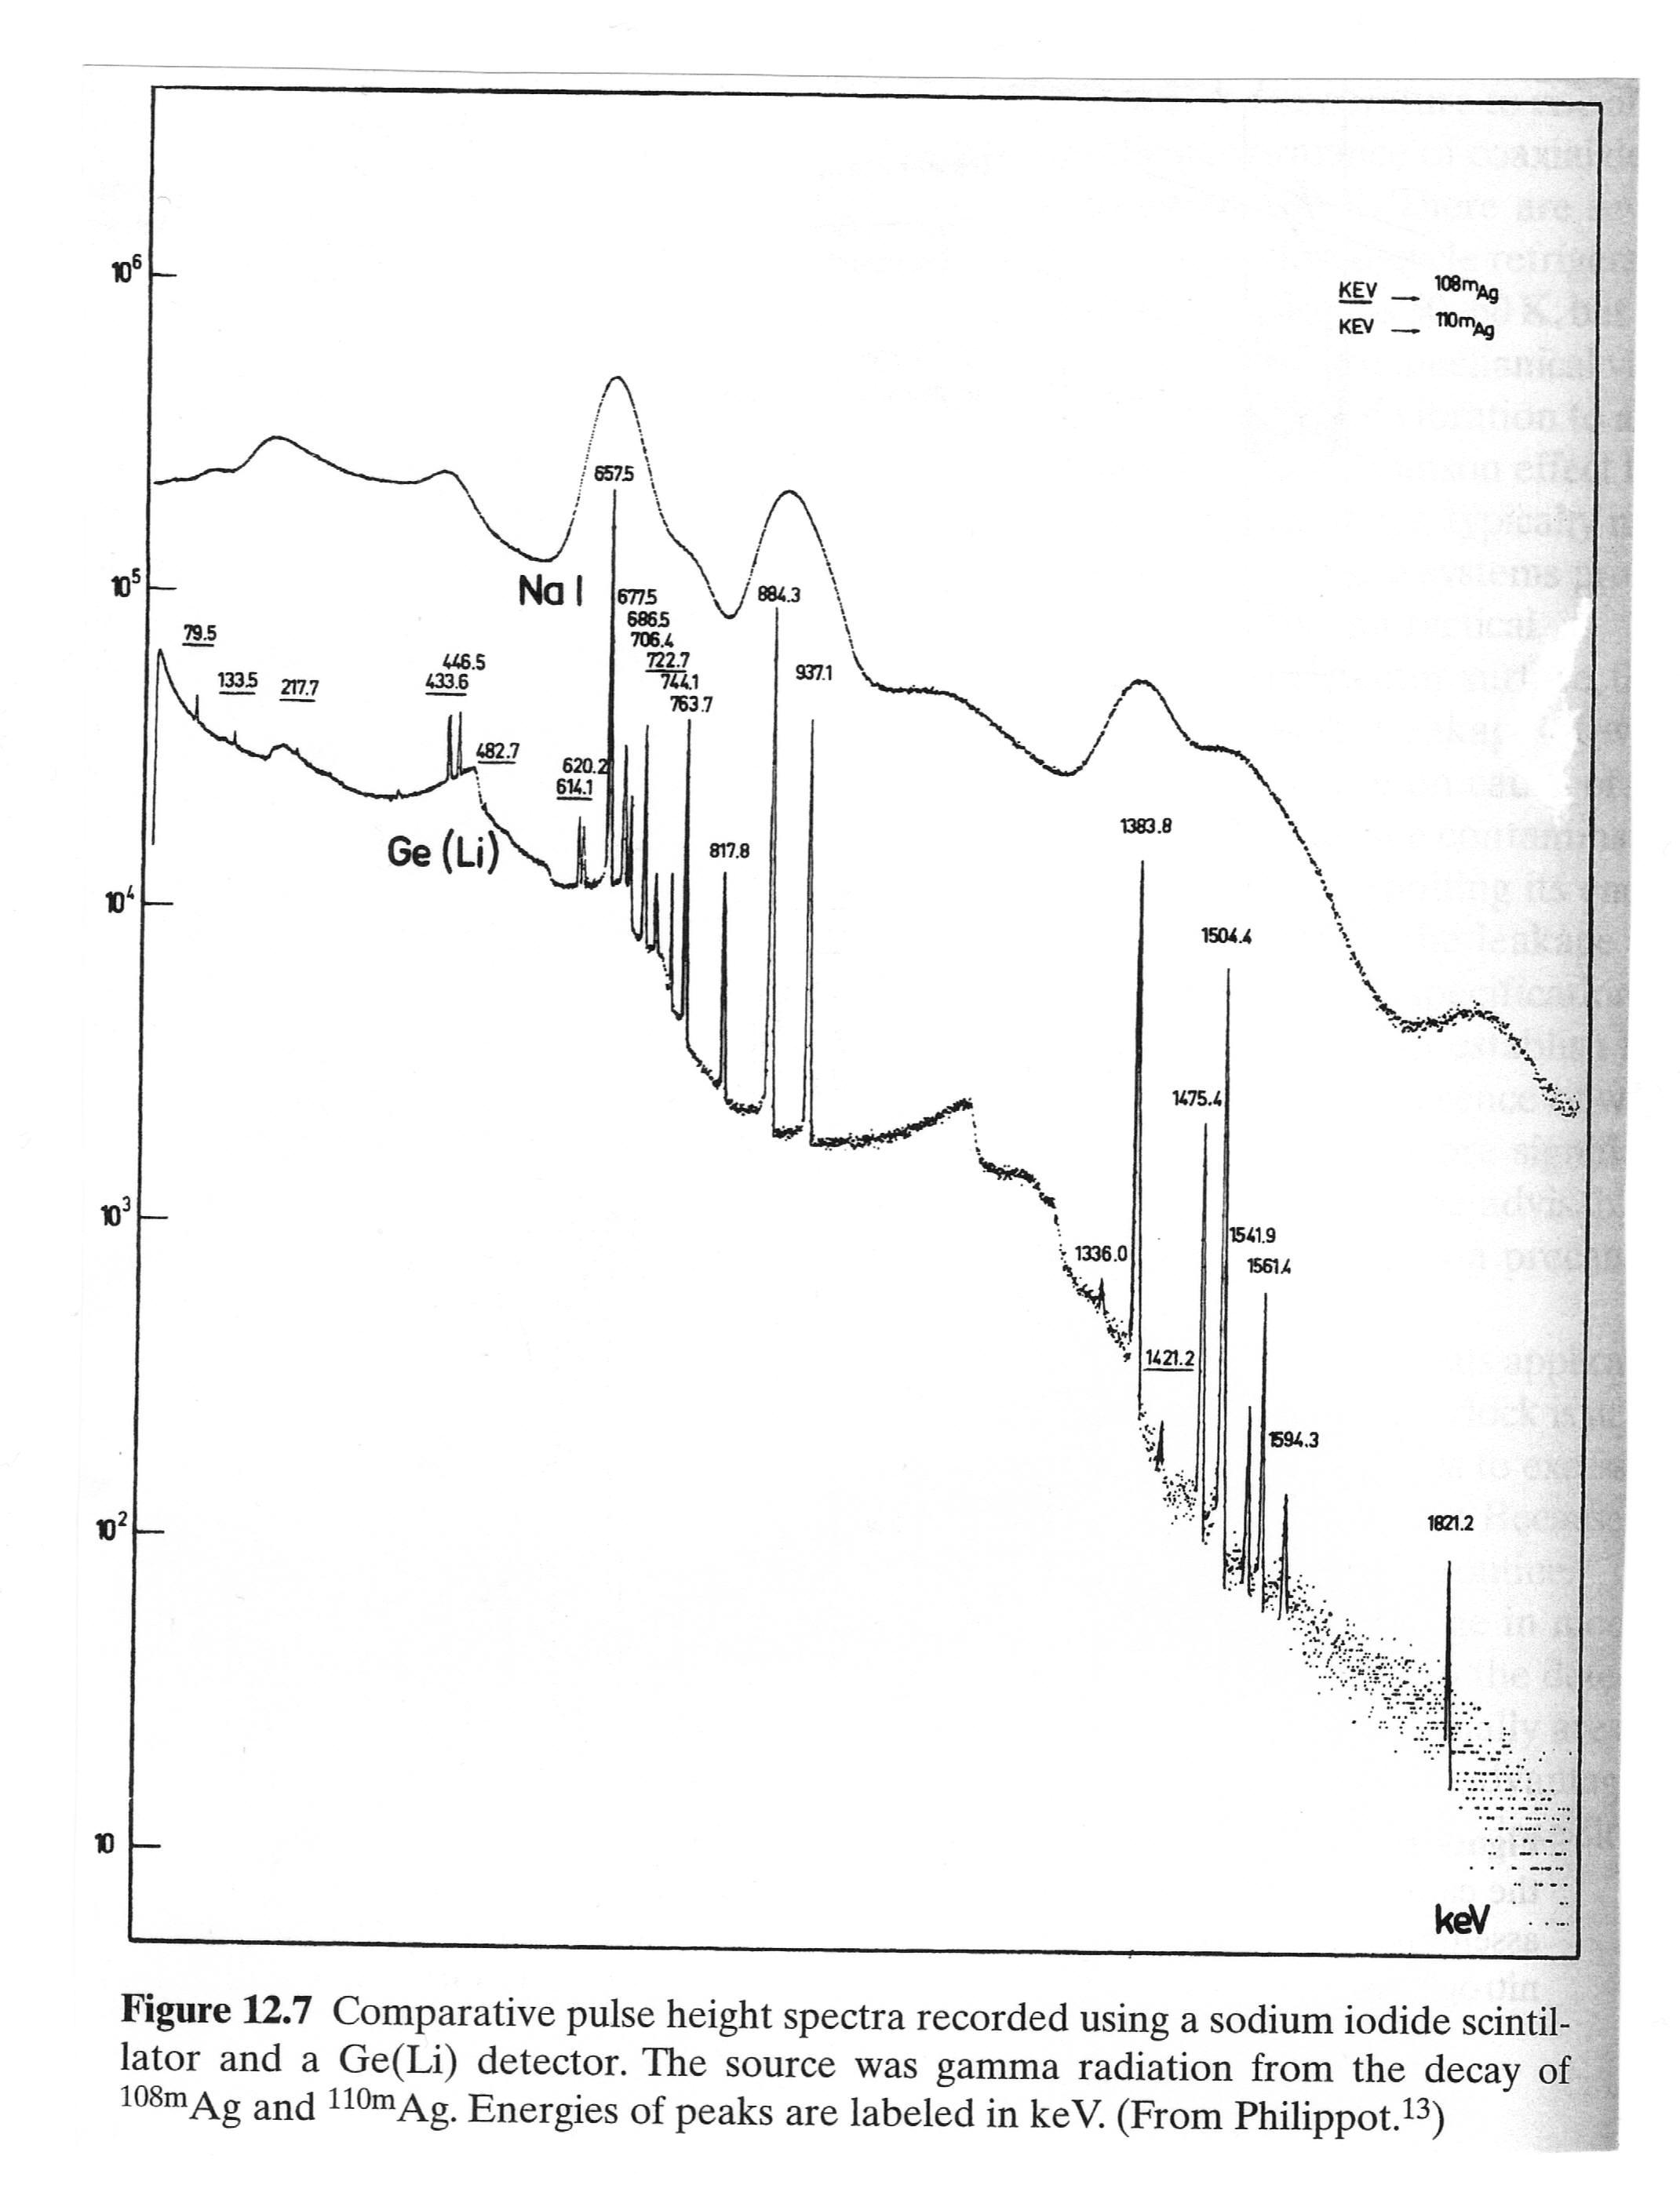
\includegraphics[width=.66\textwidth]{Plots/Energie.png}
\caption{Vergleich der Energieauflösungen von Szintillatoren und Halbleiter Detektoren. Man erkennt sehr gut, bei Halbleitern die Peaks schärfer sind und damit nahe Peaks deutlich unterscheidbar sind.}
\label{fig:energiaufloesung}
\end{figure}

Tritt nun ein Photon in diesen Detektor ein, so entsteht ein Elektron und gleichzeitg ein Loch. Elektronen können nach vorigem Kapitel nun weitere erzeugen. Durch das starke elektrische Feld werden die freien Ladungsträger nun schnell abgesaugt. Der entstandene Strom ist nun wieder direkt zu Photonenenergie proportional. Anders als zum Szintillator ist die Energieauflösunge der Germaniumdetektors größer. Dies liegt an der benötigeten Energie um Elektronen im Material zuerzeugen. Während diese im Germanium Halbleiter bei ca. $0.7eV$ liegt, benötigt man in einem NaI Szintillator fast $3eV$. \cite{energieaufloesung} Es geht viel Energie auch in Gitterschwingungen ein, welche dann nicht mehr vom PMT gemessen werden kann. Die Photonenenergie erzeugt im Szintillator nun weniger Elektronen und damit weniger Strom. Dadurch ist auch die Energieauflösung schlechter, wie in Abbildung \ref{fig:energiaufloesung} dargestellt. Es wurde die selbe radioaktive Quelle untersucht. Oben ist das Spektrum der Szintillators dargestellt, während darunter das Spektrum des Halbleiter Detektors liegt. Man erkennt sehr gut, dass einzelne Peaks oben eigentlich aus vielen einzelnen bestehen. Daher ist die Verwendung von, wie im Folgenden auch, eines Germanium Detektors sinnvoll.

Großer Nachteil, welcher in der Auswertung eine Rolle spielen wird, ist die benötigte ständige Kühlung. Damit der Germanium Detektor wie erwartet funktionieren kann benötigte er eine Temperatur von ca. $T=77K$. Dies wird mit flüssigem Stickstoff umgesetzt. Der Grund für die Wichtigkeit dieser Temperatur ist, wie auch der große Vorteil, die geringe Bandlücke des Halbleiters von $E_g=0.7eV$. Bereits bei Zimmertemperatur ist die thermische Energie im Kristall groß genug um so Elektronen Loch Paare zu erzeugen. Dieser Stromfluss wird als Rauschen wahrgenommen und überdeckt das eigentliche Spektrum der zu messenden radioaktiven Strahlung.


\newpage
\section{Experiment}
\subsection{Setup}
Wie in der Theorie bereits angesprochen wird für dieses Experiment ein mit flüssigem Stickstoff gekühlter Koaxial Germanium Detektor verwendet. Es handelt sich hierbei um eine schwach n-dotierten Germanium Zylinder mit Bohrloch. Die Wände des Bohrloches werden mit stark p-dotiertem Germanium beschichtet. Dabei entsteht bereits eine Sperrschicht, welche durch das anlegen einer Spannung von bis zu $U_0=3kV$ auf den ganzen Zylinder ausgeweitet wird. Der grobe Aufbau ist in Abbildung \ref{fig:setup} dargestellt.

\begin{figure}[H]
\centering
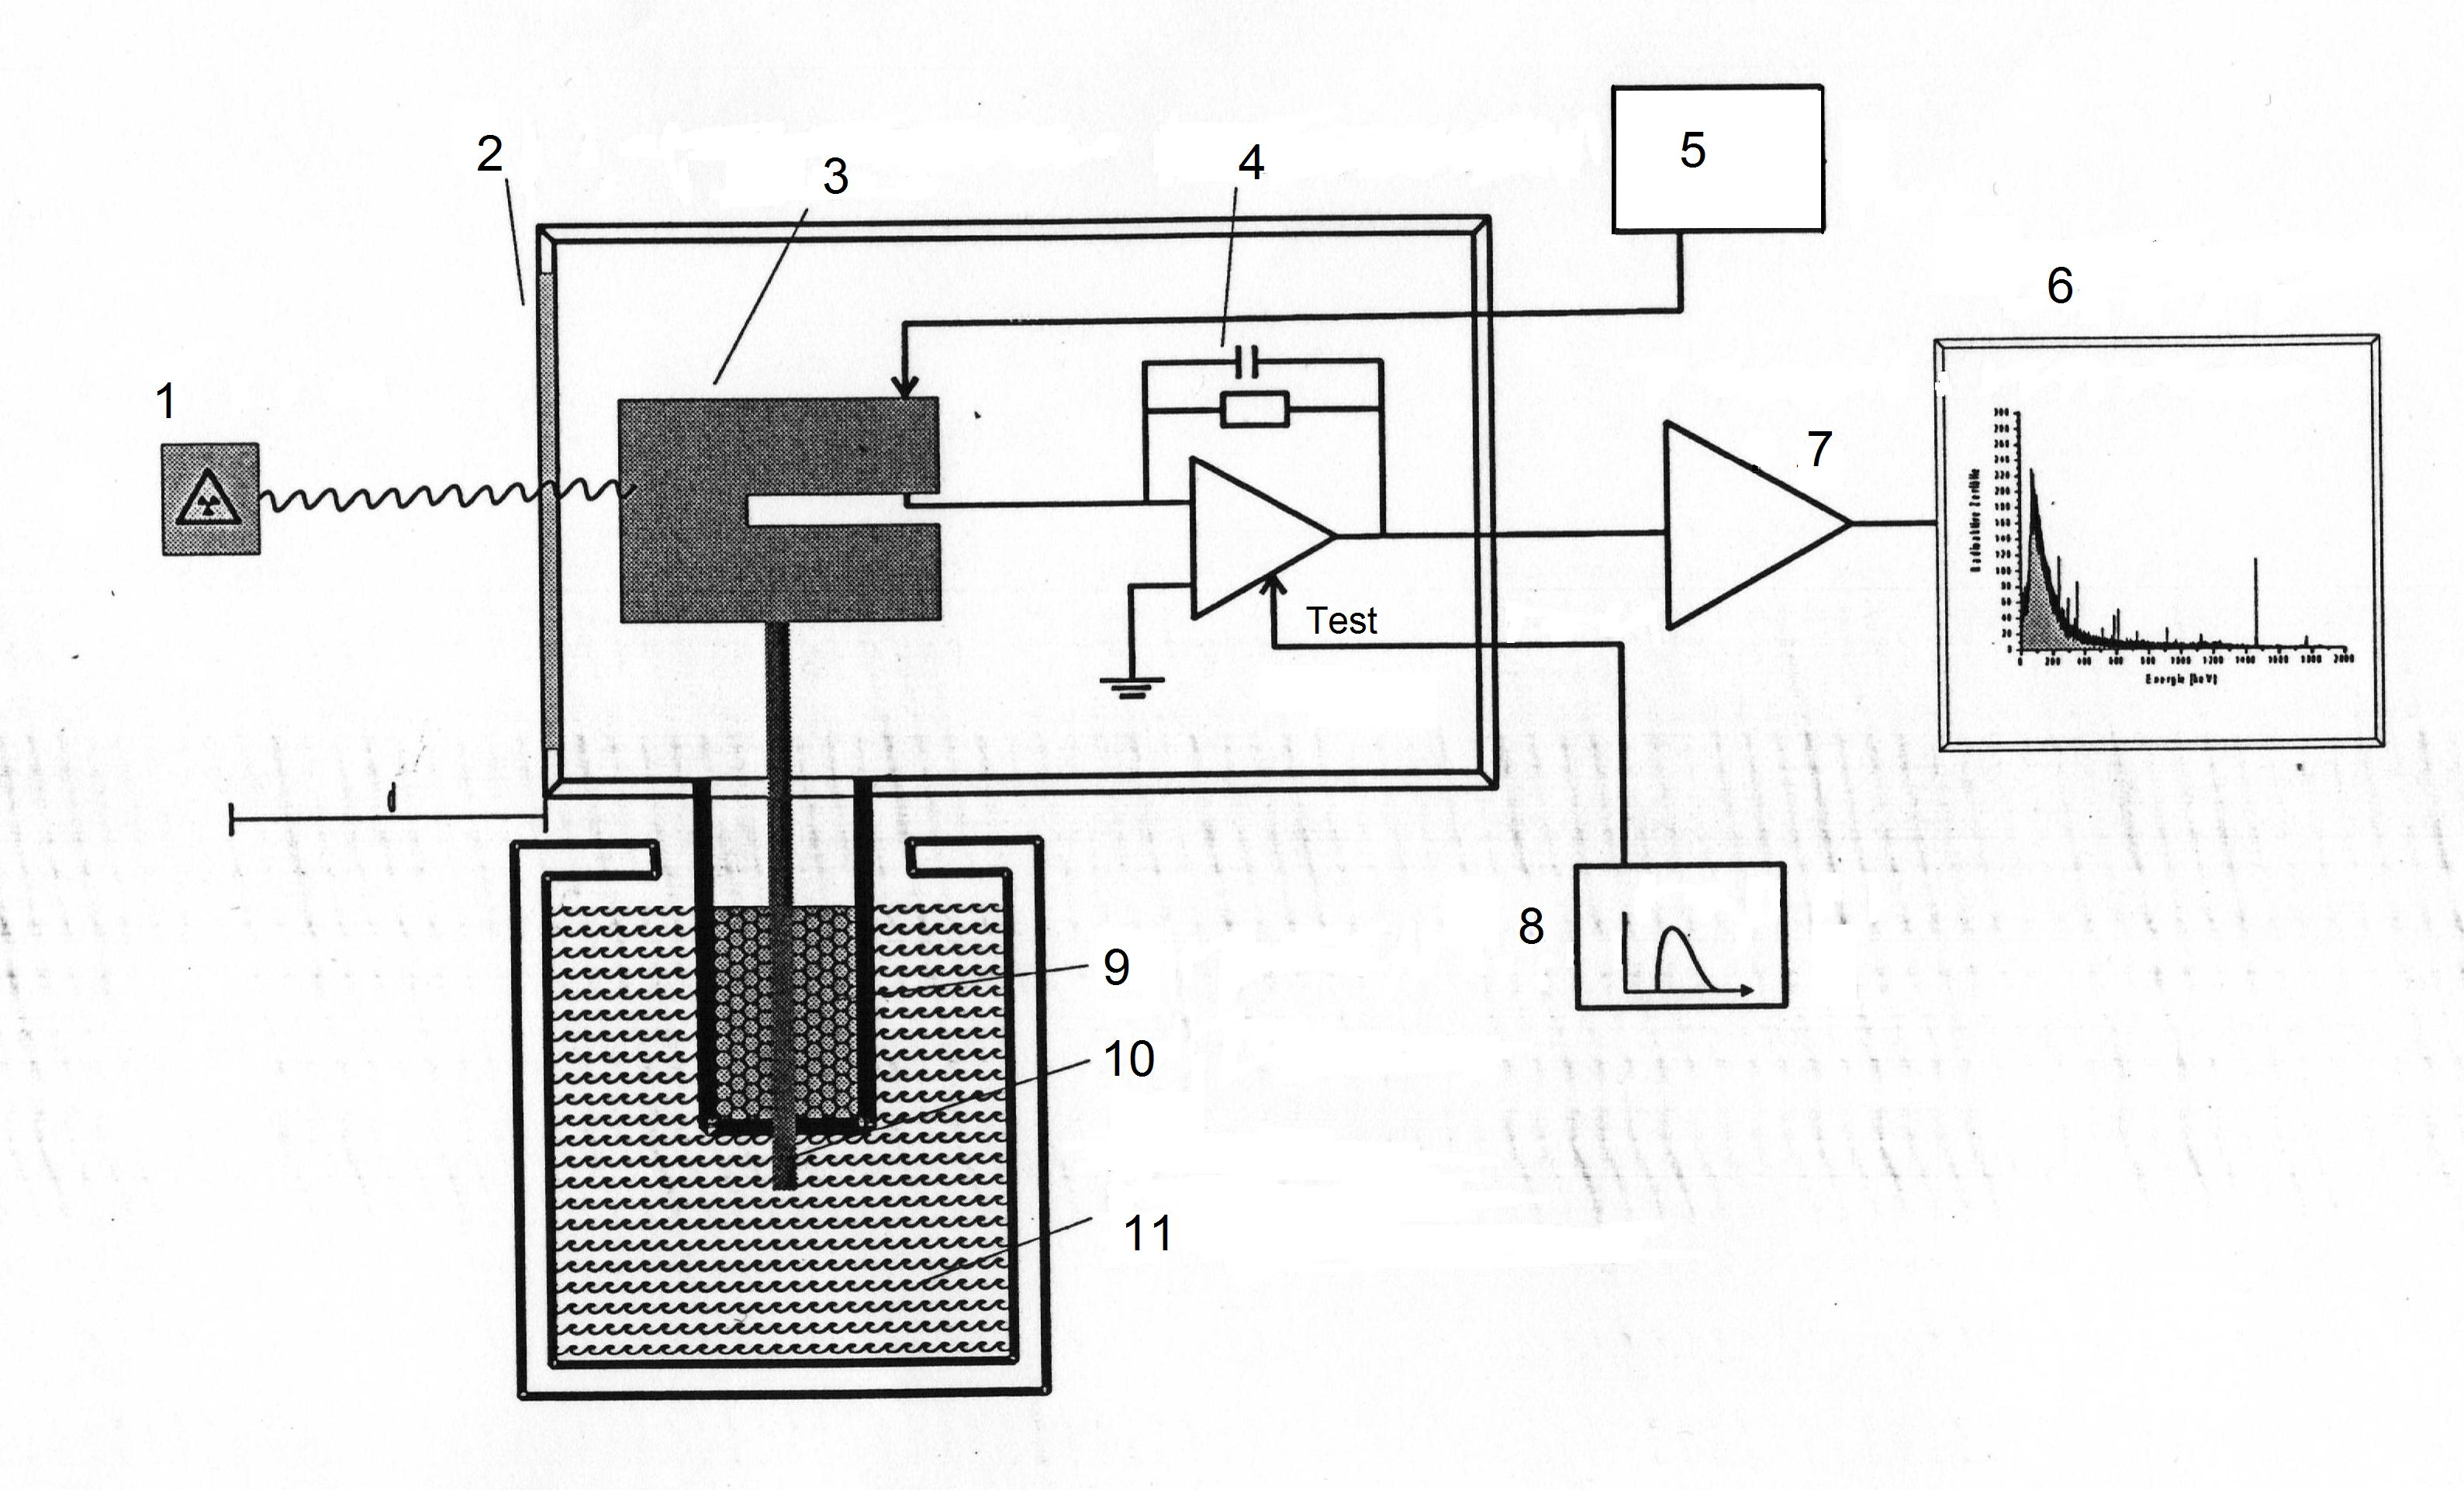
\includegraphics[width=.8\textwidth]{Plots/Setup.png}
\caption{Versuchsaufbau: 1) Radioaktive Quelle, 2) Fenster zur Vakuumkammer, 3) Germanium Detektor, 4) Preamplifier, 5) Hochspannungsquelle, 6) MCA inkl. ADC, 7) Main Amplifier, 8) Pulser, 9) Teilchensieb, 10) Kupferstab zur Kühlung, 11) Flüssiges $N_2$  }
\label{fig:setup}
\end{figure}

Die Signale werden dann vom Preamplifier verstärkt. Da es sich bei einem solchen Signal im Optimalfall um eine Delta Funktion handelt, bei der die Amplitude direkt zur Energie proportional ist. Dies kann nur schlecht elektronisch realisiert werden, daher besitzt das Ausgangssignal hier noch einen abklingenden Teil, siehe Abbildung \ref{fig:signals}. Dieser hat keine zusätzliche Information über die Energie der Strahlung sondern entsteht, da sich der Schaltkreis bzw. Operationsverstärker nicht instantan wieder entladen kann. Es entsteht hierbei also eine kurze Totzeit in welcher der Preamplifier nicht arbeiten kann. 

\begin{figure}[H]
\centering 
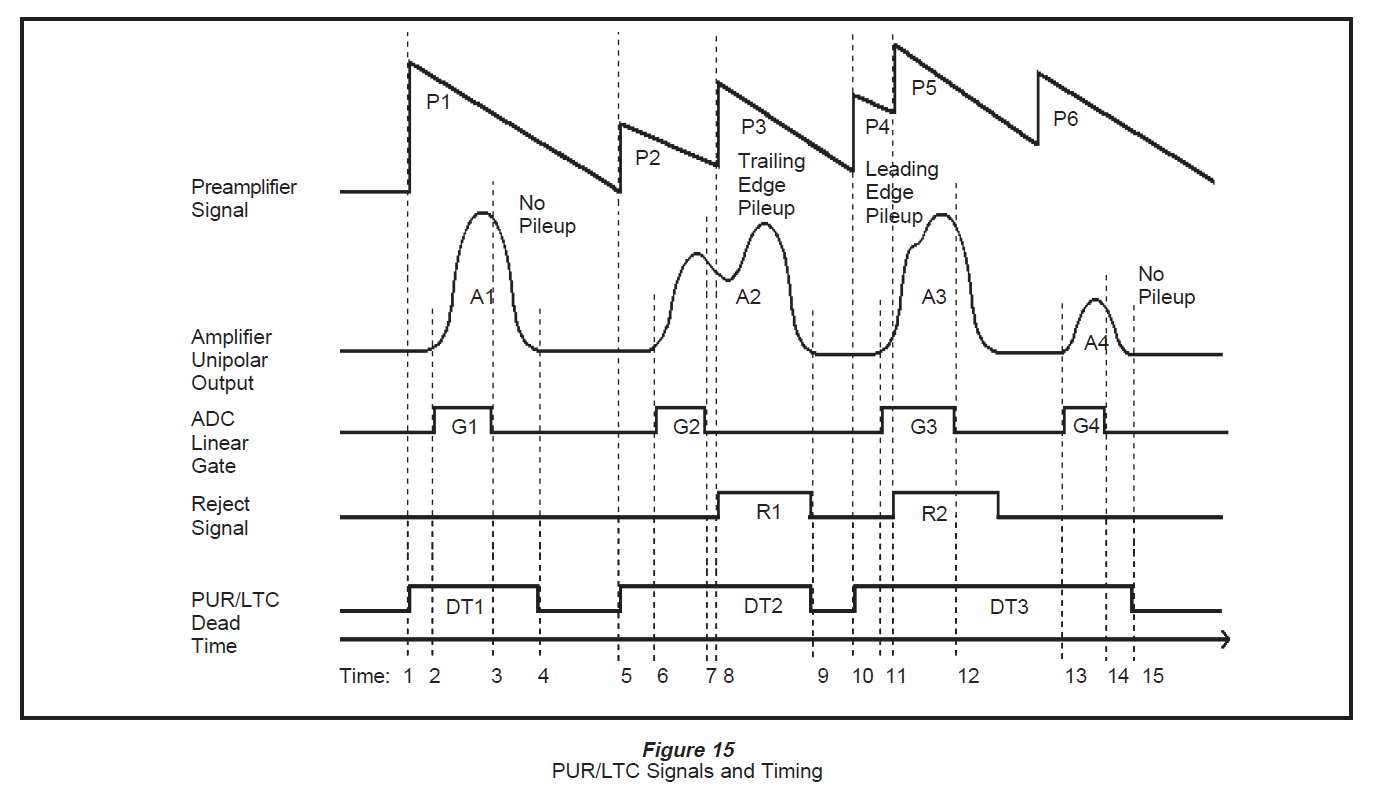
\includegraphics[width=1\textwidth]{Plots/deadtime.png}
\caption{Darstellung der Signalübertragung zwischen Preamplifier, Main Amplifier und ADC Output an den Computer. \cite{signalverarbeitung}  }
\label{fig:signals}
\end{figure}

Danach wird das Signal vom Main Amplifier umgeformt, damit der ADC dieses später in ein digitales Signal umwandeln kann. Die wichtigste Bedingung daran ist eine gemeinsame Grundlinie. Klingt das Signal wegen langsamer Kondensatorentladung nicht auf eine konstante 0 ab, so kann nicht genau bestimmt werden wann das Signal zu Ende ist. Ebenso ist es ungünstig Delta Funktionen zu messen, da das Zeitfenster zur Energiebestimmung sehr klein ist. Daher werden aus diesen Dreieck-Signalen von Main Amplifier Gausspeaks geformt. Es entspricht einer Schaltung eines Hochpasses mit folgendem Tiefpass. Der Hochpass erstellt die 0 Linie während der Tiefpass die Spitzen glättet. Weiterhin bleibt die Energieinformation im Maximum des Peaks.

Mit der Breite des Gauss kann man nun bestimmen wie schnell die Messung sein kann. Für kleine Zeitkonstanten TC, die Breite der Gausskurve entspricht $7.3\cdot TC$ \cite{signalverarbeitung}, ist der Peak nun schmal. Damit besteht die Möglichkeit mehr Events einzeln zu messen. Die Energieauflösung nimmt jedoch wegen schmalerem Signal wiederum ab. Eine Möglichkeit dies zu verhindern ist die Probe weiter vom Detektor zu platzieren, wie später noch beschrieben wird.

Es gibt nun wie in Abbildung \ref{fig:signals} gezeigt, die Möglichkeit zwei Pulse, die zu nah aneinander sind abzulehnen. Dazu benötigt man ein Ablehnungssignal (Reject Signal), welches vom ... ausgesendet wird und entscheidet ob eine gültige Messung vorliegt. Dies führt jedoch zu einer größeren Totzeit des Detektors und damit zu einer schlechten Bestimmung der Aktivität einer Quelle. In unserem Fall wird dieser Mechanismus bewusst nicht benutzt um eine Energiekalibration mit den $^{60}Co$ Peaks durchzuführen, aber auch da es für geringe Zählrate unnötig ist.  
%%%%%%%%%% REF 60Co
Die Aktivität der zu vermessenden Präparate, siehe Tabelle \ref{tab:T 1/2}, ist mit großer Wahrscheinlichkeit bereits so gering, dass die empfohlenen $25cm$ Abstand zum Detektor, nicht mehr notwendig sind. Angeblich seien diese von 1995 und damit sind alle hoch aktiven Quellen wie $^{60}Co$ und $^{22}Na$ bereits auf $2^{-20a/T_{1/2}} \approx 1/16 \ bzw. \ 1/1024 $ der ursprünglichen Menge und damit Aktivität zerfallen. Alle Materialien anderen besitzen wegen hoher Halbwertszeit sowieso nur geringe Aktivitäten. 
Daher wurden die Präparate direkt an der Vakuumkammer fixiert.

\begin{table}[H]
\centering
\begin{tabular}{c|c|c|c|c|c|c}
Präparat & $^{60}Co$& $^{133}Ba$& $^{152}Eu$& $^{137}Cs$& $^{22}Na$ & $^{241}Am$ \\ \hline 
Halbwertszeit $T_{1/2} [a]$ & 5.27 & 10.51 & 13.52 & 30.17 & 2.60 & 241.06  \\ 
\end{tabular}
\caption{Verwendete radioaktive Materialien und deren Halbwertszeit.}
\label{tab:T 1/2}
\end{table}

Zuletzt wird das Signal von Analog-To-Digital Converter (ADC) umgeformt, damit der aus dem Peak ein langes Signal wird, welches dann die Energieinformation beinhaltet. Dazu wird prinzipiell die Energie in eine Kondensator gespeichert und die Zeit der Entladung gemessen. Diese wird als Signal an den PC weitergegeben und entspricht weiterhin der Photonenenergie. Ein positives Ablehnungssignal würde die Weitergabe des Signals verhindern. Effektiv wäre dies dann keine Messung.

%%% Signal verarbietung? JA!


\newpage
\section{Anhang}


\newpage
\begin{thebibliography}{}

\bibitem{protonzerfall} \begin{verbatim}
https://de.wikipedia.org/wiki/Protonenzerfall
\end{verbatim}

\bibitem{cobalt} \begin{verbatim}
https://en.wikipedia.org/wiki/Cobalt-60
\end{verbatim}

\bibitem{energieaufloesung} 
\begin{verbatim}
Vorlesung2_11_2011.ppt , Torsten Kröll, TU Darmstadt
\end{verbatim}  

\bibitem{signalverarbeitung} 
\begin{verbatim}
Ge_Gamma_Spectroscopy.pdf , Canberra Nuclear, aus dem Wiki.
\end{verbatim}  

\end{thebibliography}
\end{document}

